\chapter{General purpose tools}
\label{seq}

\begin{enumerate}

\item \texttt{gto\char`_char\char`_to\char`_line}: it splits a sequence into lines, creating an output sequence which has a char for each line.

\item \texttt{gto\char`_reverse}: it reverses the order of a sequence.

\item \texttt{gto\char`_new\char`_line\char`_on\char`_new\char`_x}: it splits different rows with a new empty row.

\item \texttt{gto\char`_upper\char`_bound}: it sets an upper bound in a file with a value per line.

\item \texttt{gto\char`_lower\char`_bound}: it sets an lower bound in a file with a value per line.

\item \texttt{gto\char`_brute\char`_force\char`_string}: it generates all combinations, line by line, for an inputted alphabet and specific size.

\item \texttt{gto\char`_real\char`_to\char`_binary\char`_with\char`_threshold}: it converts a sequence of real numbers into a binary sequence, given a threshold.

\item \texttt{gto\char`_sum}: it adds decimal values in file, line by line, splitted by spaces or tabs.

\item \texttt{gto\char`_filter}: it filters numerical sequences.

\item \texttt{gto\char`_word\char`_search}: it search for a word in a file.

\item \texttt{gto\char`_permute\char`_by\char`_blocks}: it permutates by block sequence, FASTA and Multi-FASTA files. 

\item \texttt{gto\char`_info}: it gives the basic properties of the file, namely size, cardinality, distribution percentage of the symbols, among others.

\item \texttt{gto\char`_segment}: it segments a filtered sequence.

\item \texttt{gto\char`_comparative\char`_map}: it creates a visualization for comparative maps.

\item \texttt{gto\char`_max}: it computes the maximum value in each row between two files.

\item \texttt{gto\char`_xs}: it ...

\item \texttt{gto\char`_geco}: it ...

\item \texttt{gto\char`_gede}: it ...

\end{enumerate}

\section{Program gto\char`_char\char`_to\char`_line}
The \texttt{gto\char`_char\char`_to\char`_line} splits a sequence into lines, creating an output sequence which has a char for each line.\\
For help type:
\begin{lstlisting}
./gto_char_to_line -h
\end{lstlisting}
In the following subsections, we explain the input and output paramters.

\subsection*{Input parameters}

The \texttt{gto\char`_char\char`_to\char`_line} program needs two streams for the computation,
namely the input and output standard. The input stream is a sequence file.\\
The attribution is given according to:
\begin{lstlisting}
Usage: ./gto_char_to_line [options] [[--] args]
   or: ./gto_char_to_line [options]

It splits a sequence into lines, creating an output sequence which has a char for each line.

    -h, --help        show this help message and exit

Basic options
    < input.seq       Input sequence file (stdin)
    > output.seq      Output sequence file (stdout)

Example: ./gto_char_to_line < input.seq > output.seq
\end{lstlisting}
An example on such an input file is:
\begin{lstlisting}
ACAAGACGGCCTCCTGCTGCTGCTGCTCTCCGGGGCCACGGCCCTGGAGGGTCCACCGCTGCCCTGCTGCCATTGTCCCC
GGCCCCACCTAAGGAAAAGCAGCCTCCTGACTTTCCTCGCTTGGGCCGAGACAGCGAGCATATGCAGGAAGCGGCAGGAA
GTGGTTTGAGTGGACCTCCGGGCCCCTCATAGGAGAGGAAGCTCGGGAGGTGGCCAGGCGGCAGGAAGCAGGCCAGTGCC
GCGAATCCGCGCGCCGGGACAGAATCTCCTGCAAAGCCCTGCAGGAACTTCTTCTGGAAGACCTTCTCCACCCCCCCAGC
TAAAACCTCACCCATGAATGCTCACGCAAGTTTAATTACAGACCTGAAACAAGATGCCATTGTCCCCCGGCCTCCTGCTG
CTGCTGCTCTCCGGGGCCACGGCCACCGCTGCCCTGCCCCTGGAGGGTGGCCCCACCGGCCGAGACAGCGAGCATATGCA
GGAAGCGGCAGGAATAAGGAAAAGCAGCCTCCTGACTTTCCTCGCTTGGTGGTTTGAGTGGACCTCCCAGGCCAGTGCCG
GGCCCCTCATAGGAGAGGAAGCTCGGGAGGTGGCCAGGCGGCAGGAAGGCGCACCCCCCCAGCAATCCGCGCGCCGGGAC
AGAATGCCCTGCAGGAACTTCTTCTGGAAGACCTTCTCCTCCTGCAAATAAAACCTCACCCATGAATGCTCACGCAAGTT
TAATTACAGACCTGAA
\end{lstlisting}

\subsection*{Output}
The output of the \texttt{gto\char`_char\char`_to\char`_line} program is a group sequence splited by \textbackslash n foreach character.\\
Using the input above, an output example for this is the following:
\begin{lstlisting}
A
C
A
A
G
A
C
G
G
C
C
T
C
C
T
G
C
T
G
C
T
...
\end{lstlisting}
\section{Program gto\char`_reverse}
The \texttt{gto\char`_reverse} reverses the order of a sequence file.\\
For help type:
\begin{lstlisting}
./gto_reverse -h
\end{lstlisting}
In the following subsections, we explain the input and output paramters.

\subsection*{Input parameters}

The \texttt{gto\char`_reverse} program needs two streams for the computation,
namely the input and output standard. The input stream is a sequence file.\\
The attribution is given according to:
\begin{lstlisting}
Usage: ./gto_reverse [options] [[--] args]
   or: ./gto_reverse [options]

It reverses the order of a sequence file.

    -h, --help        show this help message and exit

Basic options
    < input.seq       Input sequence file (stdin)
    > output.seq      Output sequence file (stdout)

Example: ./gto_reverse < input.seq > output.seq
\end{lstlisting}
An example on such an input file is:
\begin{lstlisting}
ACAAGACGGCCTCCTGCTGCTGCTGCTCTCCGGGGCCACGGCCCTGGAGGGTCCACCGCTGCCCTGCTGCCATTGTCCCC
GGCCCCACCTAAGGAAAAGCAGCCTCCTGACTTTCCTCGCTTGGGCCGAGACAGCGAGCATATGCAGGAAGCGGCAGGAA
GTGGTTTGAGTGGACCTCCGGGCCCCTCATAGGAGAGGAAGCTCGGGAGGTGGCCAGGCGGCAGGAAGCAGGCCAGTGCC
GCGAATCCGCGCGCCGGGACAGAATCTCCTGCAAAGCCCTGCAGGAACTTCTTCTGGAAGACCTTCTCCACCCCCCCAGC
TAAAACCTCACCCATGAATGCTCACGCAAGTTTAATTACAGACCTGAAACAAGATGCCATTGTCCCCCGGCCTCCTGCTG
CTGCTGCTCTCCGGGGCCACGGCCACCGCTGCCCTGCCCCTGGAGGGTGGCCCCACCGGCCGAGACAGCGAGCATATGCA
GGAAGCGGCAGGAATAAGGAAAAGCAGCCTCCTGACTTTCCTCGCTTGGTGGTTTGAGTGGACCTCCCAGGCCAGTGCCG
GGCCCCTCATAGGAGAGGAAGCTCGGGAGGTGGCCAGGCGGCAGGAAGGCGCACCCCCCCAGCAATCCGCGCGCCGGGAC
AGAATGCCCTGCAGGAACTTCTTCTGGAAGACCTTCTCCTCCTGCAAATAAAACCTCACCCATGAATGCTCACGCAAGTT
TAATTACAGACCTGAA
\end{lstlisting}

\subsection*{Output}
The output of the \texttt{gto\char`_reverse} program is a group sequence.\\
Using the input above, an output example for this is the following:
\begin{lstlisting}
AAGTCCAGACATTAATTTGAACGCACTCGTAAGTACCCACTCCAAAATAAACGTCCTCCTCTTCCAGAAGGTCTTCTTCA
AGGACGTCCCGTAAGACAGGGCCGCGCGCCTAACGACCCCCCCACGCGGAAGGACGGCGGACCGGTGGAGGGCTCGAAGG
AGAGGATACTCCCCGGGCCGTGACCGGACCCTCCAGGTGAGTTTGGTGGTTCGCTCCTTTCAGTCCTCCGACGAAAAGGA
ATAAGGACGGCGAAGGACGTATACGAGCGACAGAGCCGGCCACCCCGGTGGGAGGTCCCCGTCCCGTCGCCACCGGCACC
GGGGCCTCTCGTCGTCGTCGTCCTCCGGCCCCCTGTTACCGTAGAACAAAGTCCAGACATTAATTTGAACGCACTCGTAA
GTACCCACTCCAAAATCGACCCCCCCACCTCTTCCAGAAGGTCTTCTTCAAGGACGTCCCGAAACGTCCTCTAAGACAGG
GCCGCGCGCCTAAGCGCCGTGACCGGACGAAGGACGGCGGACCGGTGGAGGGCTCGAAGGAGAGGATACTCCCCGGGCCT
CCAGGTGAGTTTGGTGAAGGACGGCGAAGGACGTATACGAGCGACAGAGCCGGGTTCGCTCCTTTCAGTCCTCCGACGAA
AAGGAATCCACCCCGGCCCCTGTTACCGTCGTCCCGTCGCCACCTGGGAGGTCCCGGCACCGGGGCCTCTCGTCGTCGTC
GTCCTCCGGCAGAACA
\end{lstlisting}
\section{Program gto\char`_new\char`_line\char`_on\char`_new\char`_x}
The \texttt{gto\char`_new\char`_line\char`_on\char`_new\char`_x} splits different rows with a new empty row.\\
For help type:
\begin{lstlisting}
./gto_new_line_on_new_x -h
\end{lstlisting}
In the following subsections, we explain the input and output paramters.

\subsection*{Input parameters}

The \texttt{gto\char`_new\char`_line\char`_on\char`_new\char`_x} program needs two streams for the computation, namely the input and output standard. The input stream is a matrix file format with 3 columns.\\
The attribution is given according to:
\begin{lstlisting}
Usage: ./gto_new_line_on_new_x [options] [[--] args]
   or: ./gto_new_line_on_new_x [options]

It splits different rows with a new empty row.

    -h, --help    show this help message and exit

Basic options
    < input       Input file with 3 column matrix format (stdin)
    > output      Output file with 3 column matrix format (stdout)

Example: ./gto_new_line_on_new_x < input > output
\end{lstlisting}
An example of such an input file is:
\begin{lstlisting}
1	2	2
1	2	2
4	4	1
10	12	2
15	15	1
45	47	3
45	47	3
45	47	3
45	47	3
55	55	1
\end{lstlisting}

\subsection*{Output}
The output of the \texttt{gto\char`_new\char`_line\char`_on\char`_new\char`_x} program is a 3 column matrix, with an empty line between different rows.\\
Using the input above, an output example for this is the following:
\begin{lstlisting}
1.000000	2.000000	2.000000
1.000000	2.000000	2.000000

4.000000	4.000000	1.000000

10.000000	12.000000	2.000000

15.000000	15.000000	1.000000

45.000000	47.000000	3.000000
45.000000	47.000000	3.000000
45.000000	47.000000	3.000000
45.000000	47.000000	3.000000

55.000000	55.000000	1.000000
\end{lstlisting}

\section{Program gto\char`_upper\char`_bound}
The \texttt{gto\char`_upper\char`_bound} sets an upper bound in a file with a value per line.\\
For help type:
\begin{lstlisting}
./gto_upper_bound -h
\end{lstlisting}
In the following subsections, we explain the input and output paramters.

\subsection*{Input parameters}

The \texttt{gto\char`_upper\char`_bound} program needs two streams for the computation,
namely the input and output standard. The input stream is a numeric file.\\
The attribution is given according to:
\begin{lstlisting}
Usage: ./gto_upper_bound [options] [[--] args]
   or: ./gto_upper_bound [options]

It sets an upper bound in a file with a value per line.

    -h, --help                show this help message and exit

Basic options
    -u, --upperbound=<int>    The upper bound value
    < input                   Input numeric file (stdin)
    > output                  Output numeric file (stdout)

Example: ./gto_upper_bound -u <upperbound> < input > output
\end{lstlisting}
An example on such an input file is:
\begin{lstlisting}
0.123
3.432
2.341
1.323
7.538
4.122
0.242
0.654
5.633
\end{lstlisting}

\subsection*{Output}
The output of the \texttt{gto\char`_upper\char`_bound} program is a set of numbers truncated at the a defined upper bound.\\
An example, for the input, is:
\begin{lstlisting}
Using upper bound: 4
0.123000
3.432000
2.341000
1.323000
4.000000
4.000000
0.242000
0.654000
4.000000
\end{lstlisting}
\section{Program gto\char`_lower\char`_bound}
The \texttt{gto\char`_lower\char`_bound} sets an lower bound in a file with a value per line.\\
For help type:
\begin{lstlisting}
./gto_lower_bound -h
\end{lstlisting}
In the following subsections, we explain the input and output paramters.

\subsection*{Input parameters}

The \texttt{gto\char`_lower\char`_bound} program needs two streams for the computation,
namely the input and output standard. The input stream is a numeric file.\\
The attribution is given according to:
\begin{lstlisting}
Usage: ./gto_lower_bound [options] [[--] args]
   or: ./gto_lower_bound [options]

It sets an lower bound in a file with a value per line.

    -h, --help                show this help message and exit

Basic options
    -u, --lowerbound=<int>    The lower bound value
    < input                   Input numeric file (stdin)
    > output                  Output numeric file (stdout)

Example: ./gto_lower_bound -u <lowerbound> < input > output
\end{lstlisting}
An example on such an input file is:
\begin{lstlisting}
0.123
3.432
2.341
1.323
7.538
4.122
0.242
0.654
5.633
\end{lstlisting}

\subsection*{Output}
The output of the \texttt{gto\char`_lower\char`_bound} program is a set of numbers truncated at the a defined lower bound.\\
Using the input above, an output example for this is the following:
\begin{lstlisting}
Using lower bound: 2
2.000000
3.432000
2.341000
2.000000
7.538000
4.122000
2.000000
2.000000
5.633000
\end{lstlisting}
\section{Program gto\char`_brute\char`_force\char`_string}
The \texttt{gto\char`_brute\char`_force\char`_string} generates all combinations, line by line, for an inputted alphabet and specific size.\\
For help type:
\begin{lstlisting}
./gto_brute_force_string -h
\end{lstlisting}
In the following subsections, we explain the input and output paramters.

\subsection*{Input parameters}

The \texttt{gto\char`_brute\char`_force\char`_string} program needs some paramenters for the computation, namely the alphabet and the key size.\\
The attribution is given according to:
\begin{lstlisting}
Usage: ./gto_brute_force_string [options] [[--] args]
   or: ./gto_brute_force_string [options]

It generates all combinations, line by line, for an inputted alphabet and specific size.

    -h, --help            show this help message and exit

Basic options
    -a, --alphabet=<str>  The input alphabet
    -s, --size=<int>      The combinations size
    > output              Output all the combinations (stdout)

Example: ./gto_brute_force_string-a <alphabet> -s <size> > output
\end{lstlisting}

\subsection*{Output}
The output of the \texttt{gto\char`_brute\char`_force\char`_string} program is a set of all possible word combinations with a defined size, using the input alphabet.\\
Using the input above with the alphabet ''abAB'' with the word size of 3, an output example for this is the following:
\begin{lstlisting}
aaa
aab
aaA
aaB
aba
...
BBb
BBA
BBB
\end{lstlisting}
\section{Program gto\char`_real\char`_to\char`_binary\char`_with\char`_threshold}
The \texttt{gto\char`_real\char`_to\char`_binary\char`_with\char`_threshold} converts a sequence of real numbers into a binary sequence, given a threshold. The numbers below to the threshold will be 0.\\
For help type:
\begin{lstlisting}
./gto_real_to_binary_with_threshold -h
\end{lstlisting}
In the following subsections, we explain the input and output paramters.

\subsection*{Input parameters}

The \texttt{gto\char`_real\char`_to\char`_binary\char`_with\char`_threshold} program needs program needs two streams for the computation, namely the real sequence as input. These numbers should be splitted by lines.\\
The attribution is given according to:
\begin{lstlisting}
Usage: ./gto_real_to_binary_with_threshold [options] [[--] args]
   or: ./gto_real_to_binary_with_threshold [options]

It converts a sequence of real numbers into a binary sequence given a threshold.

    -h, --help                show this help message and exit

Basic options
    -t, --threshold=<dbl>     The threshold in real format
    < input.num               Input numeric file (stdin)
    > output.bin              Output binary file (stdout)

Example: ./gto_real_to_binary_with_threshold -t <threshold> < input.num > output.bin
\end{lstlisting}
An example on such an input file is:
\begin{lstlisting}
12.25
1.2
5.44
5.51
7.97
2.34
8.123
\end{lstlisting}

\subsection*{Output}
The output of the \texttt{gto\char`_real\char`_to\char`_binary\char`_with\char`_threshold} program is a binary sequence.\\
An example, for the input using the threshold of 5.5, is:
\begin{lstlisting}
1
0
0
1
1
0
1
\end{lstlisting}
\section{Program gto\char`_sum}
The \texttt{gto\char`_sum} adds decimal values in file, line by line, splitted by spaces or tabs.\\
For help type:
\begin{lstlisting}
./gto_sum -h
\end{lstlisting}
In the following subsections, we explain the input and output paramters.

\subsection*{Input parameters}

The \texttt{gto\char`_sum} program needs program needs two streams for the computation, namely the input, which is a decimal file.\\
The attribution is given according to:
\begin{lstlisting}
Usage: ./gto_sum [options] [[--] args]
   or: ./gto_sum [options]

It adds decimal values in file, line by line, splitted by spaces or tabs.

    -h, --help        show this help message and exit

Basic options
    < input.num       Input numeric file (stdin)
    > output.num      Output numeric file (stdout)

Optional
    -r, --sumrows     When active, the application adds all the values line by line
    -a, --sumall      When active, the application adds all values

Example: ./gto_sum -a < input.num > output.num
\end{lstlisting}
An example on such an input file is:
\begin{lstlisting}
0.123	5	5
3.432
2.341   3   2
1.323
7.538	5
4.122
0.242 
0.654
5.633	10
\end{lstlisting}

\subsection*{Output}
The output of the \texttt{gto\char`_sum} program is a sum of the elements in the input file.\\
Executing the application with the provided input and with the flag to add only the elements in each row (-r), the output of this execution is:
\begin{lstlisting}
10.123000
3.432000
7.341000
1.323000
12.538000
4.122000
0.242000
0.654000
15.633000
\end{lstlisting}
\section{Program gto\char`_filter}
The \texttt{gto\char`_filter} filters numerical sequences.\\
For help type:
\begin{lstlisting}
./gto_filter -h
\end{lstlisting}
In the following subsections, we explain the input and output paramters.

\subsection*{Input parameters}

The \texttt{gto\char`_filter} program needs program needs two streams for the computation, namely the input, which is a decimal file.\\
The attribution is given according to:
\begin{lstlisting}
Usage: ./gto_filter [options] [[--] args]
   or: ./gto_filter [options]

It filters numerical sequences.

    -h, --help                show this help message and exit

Basic options
    < input.num               Input numeric file (stdin)
    > output.num              Output numeric file (stdout)

Optional
    -w, --windowsize=<int>    Window size (defaut 0)
    -d, --drop=<int>          Discard elements (default 0.0)
    -t, --windowtype=<int>    Window type (0=Hamm, 1=Hann, 2=Black, 3=rec) (default 0 (Hamm))
    -c, --onecolumn           Read from one column
    -p, --printone            Print one column
    -r, --reverse             Reverse mode

Example: ./gto_filter -w <windowsize> -d <drop> -t <windowtype> -c -p -r < input.num > output.num
\end{lstlisting}
An example on such an input file is:
\begin{lstlisting}
TO DO
\end{lstlisting}

\subsection*{Output}
The output of the \texttt{gto\char`_filter} program is ...\\
An example, for the input, is:
\begin{lstlisting}
TO DO
\end{lstlisting}
\section{Program gto\char`_word\char`_search}
The \texttt{gto\char`_word\char`_search} search for a word in a file. It is case sensitive.\\
For help type:
\begin{lstlisting}
./gto_word_search -h
\end{lstlisting}
In the following subsections, we explain the input and output paramters.

\subsection*{Input parameters}

The \texttt{gto\char`_word\char`_search} program needs program needs two streams for the computation, namely the input and output standard. The input stream is a text file.\\
The attribution is given according to:
\begin{lstlisting}
Usage: ./gto_word_search [options] [[--] args]
   or: ./gto_word_search [options]

Searching for a word in a text file. It is case sensitive.

    -h, --help        show this help message and exit

Basic options
    -w, --word=<str>  Word to search in the file
    < input.txt       Input text file (stdin)
    > output.txt      Output text file (stdout)

Example: ./gto_word_search-w <word> < input.txt > output.txt
\end{lstlisting}
An example on such an input file is:
\begin{lstlisting}
No guts, no story. Chris Brady
My life is my message. Mahatma Gandhi
Screw it, let’s do it. Richard Branson
Boldness be my friend. William Shakespeare
Keep going. Be all in. Bryan Hutchinson
My life is my argument. Albert Schweitzer
Fight till the last gasp. William Shakespeare
Leave no stone unturned. Euripides
\end{lstlisting}

\subsection*{Output}
The output of the \texttt{gto\char`_word\char`_search} program is a text file with the matching paragraphs and the location of the word found.\\
Using the input above with the word ''Shakespeare'', an output example for this is the following:
\begin{lstlisting}
Found match in range [ 1536 : 2048 ]
Boldness be my friend. William Shakespeare

Found match in range [ 3072 : 3584 ]
Fight till the last gasp. William Shakespeare
\end{lstlisting}
\section{Program gto\char`_permute\char`_by\char`_blocks}
The \texttt{gto\char`_permute\char`_by\char`_blocks} permutates by block sequence, FASTA and Multi-FASTA files.\\
For help type:
\begin{lstlisting}
./gto_ -h
\end{lstlisting}
In the following subsections, we explain the input and output paramters.

\subsection*{Input parameters}

The \texttt{gto\char`_permute\char`_by\char`_blocks} program needs two streams for the computation, namely the input and output standard. The input stream is a sequence, FASTA or Multi-FASTA file.\\
The attribution is given according to:
\begin{lstlisting}
Usage: ./gto_permute_by_blocks [options] [[--] args]
   or: ./gto_permute_by_blocks [options]

It permutates by block sequence, FASTA and Multi-FASTA files.

    -h, --help            show this help message and exit

Basic options
    -b, --numbases=<int>  The number of bases in each block
    -s, --seed=<int>      Starting point to the random generator
    < input               Input sequence, FASTA or Multi-FASTA file format (stdin)
    > output              Output sequence, FASTA or Multi-FASTA file format (stdout)

Example: ./gto_permute_by_blocks -b <numbases> -s <seed> < input.fasta > output.fasta
\end{lstlisting}
An example of such an input file is:
\begin{lstlisting}
>AB000264 |acc=AB000264|descr=Homo sapiens mRNA 
ACAAGACGGCCTCCTGCTGCTGCTGCTCTCCGGGGCCACGGCCCTGGAGGGTCCACCGCTGCCCTGCTGCCATTGTCCCC
GGCCCCACCTAAGGAAAAGCAGCCTCCTGACTTTCCTCGCTTGGGCCGAGACAGCGAGCATATGCAGGAAGCGGCAGGAA
GTGGTTTGAGTGGACCTCCGGGCCCCTCATAGGAGAGGAAGCTCGGGAGGTGGCCAGGCGGCAGGAAGCAGGCCAGTGCC
GCGAATCCGCGCGCCGGGACAGAATCTCCTGCAAAGCCCTGCAGGAACTTCTTCTGGAAGACCTTCTCCACCCCCCCAGC
TAAAACCTCACCCATGAATGCTCGCAACACGCAAGTTTAATTCGCAAGTTAGACCTGAACGGGAGGTGGCCACGCAAGTT
\end{lstlisting}

\subsection*{Output}
The output of the \texttt{gto\char`_permute\char`_by\char`_blocks} program is a sequence, FASTA or Multi-FASTA file permuted following some parameters.\\
Using the input above with the base number as 80, an output example for this is the following:
\begin{lstlisting}
GGCCCCACCTAAGGAAAAGCAGCCTCCTGACTTTCCTCGCTTGGGCCGAGACAGCGAGCATATGCAGGAAGCGGCAGGAA
GTGGTTTGAGTGGACCTCCGGGCCCCTCATAGGAGAGGAAGCTCGGGAGGTGGCCAGGCGGCAGGAAGCAGGCCAGTGCC
GCGAATCCGCGCGCCGGGACAGAATCTCCTGCAAAGCCCTGCAGGAACTTCTTCTGGAAGACCTTCTCCACCCCCCCAGC
ACAAGACGGCCTCCTGCTGCTGCTGCTCTCCGGGGCCACGGCCCTGGAGGGTCCACCGCTGCCCTGCTGCCATTGTCCCC
TAAAACCTCACCCATGAATGCTCGCAACACGCAAGTTTAATTCGCAAGTTAGACCTGAACGGGAGGTGGCCACGCAAGTT
\end{lstlisting}
\section{Program gto\char`_info}
The \texttt{gto\char`_info} gives the basic properties of the file, namely size, cardinality, distribution percentage of the symbols, among others.\\
For help type:
\begin{lstlisting}
./gto_info -h
\end{lstlisting}
In the following subsections, we explain the input and output paramters.

\subsection*{Input parameters}

The \texttt{gto\char`_info} program needs two streams for the computation,
namely the input and output standard. The input stream is a file withou any specific format.\\
The attribution is given according to:
\begin{lstlisting}
Usage: ./gto_info [options] [[--] args]
   or: ./gto_info [options]

It gives the basic properties of the file, namely size, cardinality, distribution 
percentage of the symbols, among others.

    -h, --help    show this help message and exit

Basic options
    < input       Input file (stdin)
    > output      Output read information (stdout)

Optional
    -a, --ascii   When active, the application shows the ASCII codes

Example: ./gto_info < input > output

Output example :
Number of symbols  : value
Alphabet size      : value
Alphabet           : value
Symbol distribution:
<Symbol/Code ASCII>  <Symbol count>  <Distribution percentage>
\end{lstlisting}
An example on such an input file is:
\begin{lstlisting}
>AB000264 |acc=AB000264|descr=Homo sapiens mRNA 
ACAAGACGGCCTCCTGCTGCTGCTGCTCTCCGGGGCCACGGCCCTGGAGGGTCCACCGCTGCCCTGCTGCCATTGTCCCC
GGCCCCACCTAAGGAAAAGCAGCCTCCTGACTTTCCTCGCTTGGGCCGAGACAGCGAGCATATGCAGGAAGCGGCAGGAA
GTGGTTTGAGTGGACCTCCGGGCCCCTCATAGGAGAGGAAGCTCGGGAGGTGGCCAGGCGGCAGGAAGCAGGCCAGTGCC
GCGAATCCGCGCGCCGGGACAGAATCTCCTGCAAAGCCCTGCAGGAACTTCTTCTGGAAGACCTTCTCCACCCCCCCAGC
TAAAACCTCACCCATGAATGCTCGCAACACGCAAGTTTAATTCGCAAGTTAGACCTGAACGGGAGGTGGCCACGCAAGTT
\end{lstlisting}

\subsection*{Output}
The output of the \texttt{gto\char`_info} program is a set of information related to the file read. \\
Using the input above, an output example for this is the following:
\begin{lstlisting}
Number of symbols  : 453
Alphabet size      : 28
Alphabet           :|srponmiedcaTRNHGCBA>=6420 \n
Symbol distribution:
|  : 	2		0.4415011
s  : 	3		0.66225166
r  : 	1		0.22075055
p  : 	1		0.22075055
o  : 	2		0.4415011
n  : 	1		0.22075055
m  : 	2		0.4415011
i  : 	1		0.22075055
e  : 	2		0.4415011
d  : 	1		0.22075055
c  : 	3		0.66225166
a  : 	2		0.4415011
T  : 	66		14.569536
R  : 	1		0.22075055
N  : 	1		0.22075055
H  : 	1		0.22075055
G  : 	117		25.827815
C  : 	131		28.918322
B  : 	2		0.4415011
A  : 	89		19.646799
>  : 	1		0.22075055
=  : 	2		0.4415011
6  : 	2		0.4415011
4  : 	2		0.4415011
2  : 	2		0.4415011
0  : 	6		1.3245033
   : 	4		0.88300221
\n : 	5		1.1037528
\end{lstlisting}

\section{Program gto\char`_segment}
The \texttt{gto\char`_segment} segments a filtered sequence.\\
For help type:
\begin{lstlisting}
./gto_segment -h
\end{lstlisting}
In the following subsections, we explain the input and output paramters.

\subsection*{Input parameters}

The \texttt{gto\char`_segment} program needs two streams for the computation, namely the input and output standard. The input stream is a numeric file.\\
The attribution is given according to:
\begin{lstlisting}
Usage: ./gto_segment [options] [[--] args]
   or: ./gto_segment [options]

It segments a filtered sequence.

    -h, --help                show this help message and exit

Basic options
    -t, --threshold=<dbl>     The segment threshold
    < input.num               Input numeric file (stdin)
    > output                  Output the segment file (stdout)

Example: ./gto_segment -t <threshold> < input.num > output
\end{lstlisting}
An example on such an input file is:
\begin{lstlisting}
1   1.77
5   2.18
10  2.32
15  3.15
20  2.52
25  4.43
30  1.23
\end{lstlisting}

\subsection*{Output}
The output of the \texttt{gto\char`_segment} program is the interval of values ​​below the threshold.\\
An example, for the input using a thresould of 3, is:
\begin{lstlisting}
0:10
\end{lstlisting}
\section{Program gto\char`_comparative\char`_map}
The \texttt{gto\char`_comparative\char`_map} creates a visualization for comparative maps.\\
For help type:
\begin{lstlisting}
./gto_comparative_map -h
\end{lstlisting}
In the following subsections, we explain the input and output paramters.

\subsection*{Input parameters}

The \texttt{gto\char`_comparative\char`_map} program needs an input file with the plot positions, respecting a defined structure.\\
The attribution is given according to:
\begin{lstlisting}
Usage: ./gto_comparative_map [options] [[--] args]                        
   or: ./gto_comparative_map [options]                                    
                                                                          
It creates a visualization for comparative maps.                          
                                                                          
    -h, --help            Show this help message and exit                 
                                                                          
Basic options                                                             
    <FILE>                Contigs filename with positions (.pos),         
                                                                          
Optional                                                                  
                                                                          
    -h                    Give this help,                                 
    -V                    Display version number,                         
    -v                    Verbose mode (more information),                
    -l <link>             Link type between maps [0;4],                   
    -w <width>            Chromosome width,                               
    -s <space>            Space between chromosomes,                      
    -m <mult>             Color id multiplication factor,                 
    -b <begin>            Color id beggining,                             
    -c <minimum>          Minimum block size to consider,                 
    -i                    Do NOT show inversion maps,                     
    -r                    Do NOT show regular maps,                       
    -o <FILE>             Output image filename with map,                 
                                                                          
Example: ./gto_comparative_map -o map.svg map.config 
\end{lstlisting}
The input file needs to have the following structure:
\begin{lstlisting}
todo
\end{lstlisting}
An example of such an input file is:
\begin{lstlisting}
#SCF    5000000 5000000
aaa     1       1000000 1       1000000 bbbb    3000000 4000000 3000000 4000000
bbb     1500000 2000000 1500000 2000000 cccc    1500000 2000000 1500000 2000000
aaa     2000000 3000000 2000000 3000000 bbbb    3000000 2000000 3000000 2000000
\end{lstlisting}

\subsection*{Output}
The output of the \texttt{gto\char`_comparative\char`_map} program is a executing report, and a svg plot with the maps.\\
Using the input above, an output example for this is the following:
\begin{lstlisting}
==[ PROCESSING ]====================
Printing plot ...
Found 2 regular regions. 
Found 1 inverted regions.
Done!                       

==[ STATISTICS ]====================
Total cpu time: 0 second(s).
\end{lstlisting}

In the Figure~\ref{fig:gtoComparativeMap} is represented the plot for the execution above.

 \begin{figure}[!h]
  \centering
  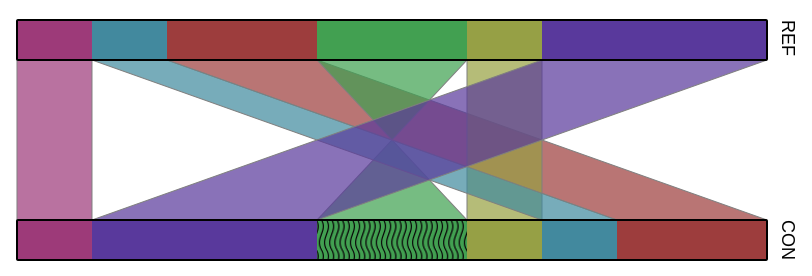
\includegraphics[scale=0.6]{./images/gto_comparative_map.png}
  \caption{\texttt{gto\char`_comparative\char`_map} execution plot.}
  \label{fig:gtoComparativeMap}
 \end{figure}
\section{Program gto\char`_max}
The \texttt{gto\char`_max} computes the maximum value in each row between two files.\\
For help type:
\begin{lstlisting}
./gto_max -h
\end{lstlisting}
In the following subsections, we explain the input and output paramters.

\subsection*{Input parameters}

The \texttt{gto\char`_max} program needs program needs two streams for the computation, namely the input, which are two decimal files.\\
The attribution is given according to:
\begin{lstlisting}
Usage: ./gto_max [options] [[--] args]
   or: ./gto_max [options]

It computes the maximum value in each row between two files.

    -h, --help                Show this help message and exit

Basic options
    -f, --first_file=<str>    File to compute the max
    -s, --second_file=<str>   The second file to do the max computation
    > output.num              Output numeric file (stdout)

Example: ./gto_max -f input1.num -s input2.num > output.num
\end{lstlisting}
An example of such an input files are:\\
File 1:
\begin{lstlisting}
0.123
3.432
2.341
1.323
7.538
4.122
0.242
0.654
5.633
\end{lstlisting}
File 2:
\begin{lstlisting}
2.123
5.312
2.355
0.124
1.785
3.521
0.532
7.324
2.312
\end{lstlisting}

\subsection*{Output}
The output of the \texttt{gto\char`_max} program is the numeric file with the maximum value for each row between both input files.\\
Executing the application with the provided input, the output of this execution is:
\begin{lstlisting}
2.123000
5.312000
2.355000
1.323000
7.538000
4.122000
0.532000
7.324000
5.633000
\end{lstlisting}
\section{Program gto\char`_xs}
The \texttt{gto\char`_xs} .\\
For help type:
\begin{lstlisting}
./gto_xs -h
\end{lstlisting}
In the following subsections, we explain the input and output paramters.

\subsection*{Input parameters}

The \texttt{gto\char`_xs} program needs program needs two streams for the computation, namely the input and output standard. ...\\
The attribution is given according to:
\begin{lstlisting}
TODO
\end{lstlisting}
An example on such an input file is:
\begin{lstlisting}
TO DO
\end{lstlisting}

\subsection*{Output}
The output of the \texttt{gto\char`_xs} program is ...\\
An example, for the input, is:
\begin{lstlisting}
TO DO
\end{lstlisting}
\section{Program gto\char`_genomic\char`_compressor}
The \texttt{gto\char`_genomic\char`_compressor} is able to provide additional compression gains over several top specific tools, while as an analysis tool, it is able to determine absolute measures, namely for many distance computations, and local measures, such as the information content contained in each element, providing a way to quantify and locate specific genomic events.\\
For help type:
\begin{lstlisting}
./gto_genomic_compressor -h
\end{lstlisting}
In the following subsections, we explain the input and output paramters.

\subsection*{Input parameters}

The \texttt{gto\char`_genomic\char`_compressor} program needs a sequence to compress.\\
The attribution is given according to:
\begin{lstlisting}
SYNOPSIS                                                                
      ./gto_genomic_compressor [OPTION]... -r [FILE] [FILE]:[FILE]:[FILE]:[...]          
                                                                        
SAMPLE                                                                  
      Run Compression         :  ./gto_genomic_compressor -v -l 3 sequence.txt           
      Run Decompression       :  ./gto_genomic_decompressor -v sequence.txt.co             
      Run Information Profile :  ./gto_genomic_compressor -v -l 3 -e sequence.txt        
                                                                        
DESCRIPTION                                                             
      Compress and decompress genomic sequences for storage purposes.   
      Measure an upper bound of the sequences entropy.                  
      Compute information profiles of genomic sequences.                
                                                                        
      -h,  --help                                                       
           usage guide (help menu).                                     
                                                                        
      -V,  --version                                                    
           Display program and version information.                     
                                                                        
      -F,  --force                                                      
           force mode. Overwrites old files.                            
                                                                        
      -v,  --verbose                                                    
           verbose mode (more information).                             
                                                                        
      -x,  --examples                                                   
           show several running examples (parameter examples).          
                                                                        
      -s,  --show-levels                                                
           show pre-computed compression levels (configured parameters).
                                                                        
      -e,  --estimate                                                   
           it creates a file with the extension ".iae" with the       
           respective information content. If the file is FASTA or      
           FASTQ it will only use the "ACGT" (genomic) sequence.      
                                                                        
      -l [NUMBER],  --level [NUMBER]                                    
           Compression level (integer).                                 
           Default level: 5.                                           
           It defines compressibility in balance with computational     
           resources (RAM & time). Use -s for levels perception.        
                                                                        
      -tm [NB_C]:[NB_D]:[NB_I]:[NB_H]:[NB_G]/[NB_S]:[NB_E]:[NB_A]       
           Template of a target context model.                          
           Parameters:                                                  
           [NB_C]: (integer [1;20]) order size of the regular context   
                   model. Higher values use more RAM but, usually, are  
                   related to a better compression score.               
           [NB_D]: (integer [1;5000]) denominator to build alpha, which 
                   is a parameter estimator. Alpha is given by 1/[NB_D].
                   Higher values are usually used with higher [NB_C],   
                   and related to confiant bets. When [NB_D] is one,    
                   the probabilities assume a Laplacian distribution.   
           [NB_I]: (integer {0,1,2}) number to define if a sub-program  
                   which addresses the specific properties of DNA       
                   sequences (Inverted repeats) is used or not. The     
                   number 2 turns ON this sub-program without the       
                   regular context model (only inverted repeats). The   
                   number 1 turns ON the sub-program using at the same  
                   time the regular context model. The number 0 does    
                   not contemple its use (Inverted repeats OFF). The    
                   use of this sub-program increases the necessary time 
                   to compress but it does not affect the RAM.          
           [NB_H]: (integer [1;254]) size of the cache-hash for deeper  
                   context models, namely for [NB_C] > 14. When the     
                   [NB_C] <= 14 use, for example, 1 as a default. The   
                   RAM is highly dependent of this value (higher value  
                   stand for higher RAM).                               
           [NB_G]: (real [0;1)) real number to define gamma. This value 
                   represents the decayment forgetting factor of the    
                   regular context model in definition.                 
           [NB_S]: (integer [0;20]) maximum number of editions allowed  
                   to use a substitutional tolerant model with the same 
                   memory model of the regular context model with       
                   order size equal to [NB_C]. The value 0 stands for   
                   turning the tolerant context model off. When the     
                   model is on, it pauses when the number of editions   
                   is higher that [NB_C], while it is turned on when    
                   a complete match of size [NB_C] is seen again. This  
                   is probabilistic-algorithmic model very usefull to   
                   handle the high substitutional nature of genomic     
                   sequences. When [NB_S] > 0, the compressor used more 
                   processing time, but uses the same RAM and, usually, 
                   achieves a substantial higher compression ratio. The 
                   impact of this model is usually only noticed for     
                   [NB_C] >= 14.                                        
           [NB_E]: (integer [1;5000]) denominator to build alpha for    
                   substitutional tolerant context model. It is         
                   analogous to [NB_D], however to be only used in the  
                   probabilistic model for computing the statistics of  
                   the substitutional tolerant context model.           
           [NB_A]: (real [0;1)) real number to define gamma. This value 
                   represents the decayment forgetting factor of the    
                   substitutional tolerant context model in definition. 
                   Its definition and use is analogus to [NB_G].        
                                                                        
      ... (you may use several target models with custom parameters)    
                                                                        
      -rm [NB_C]:[NB_D]:[NB_I]:[NB_H]:[NB_G]/[NB_S]:[NB_E]:[NB_A]       
           Template of a reference context model.                       
           Use only when -r [FILE] is set (referential compression).    
           Parameters: the same as in -tm.                              
                                                                        
      ... (you may use several reference models with custom parameters) 
                                                                        
      -r [FILE], --reference [FILE]                                     
           Reference sequence filename ("-rm" are trainned here).     
           Example: -r file1.txt.                                       
                                                                        
      [FILE]                                                            
           Input sequence filename (to compress) -- MANDATORY.          
           File(s) to compress (last argument).                         
           For more files use splitting ":" characters.               
           Example: file1.txt:file2.txt:file3.txt.
\end{lstlisting}
In the following example, it will be downloaded seventeen DNA sequences, and compress and decompress one of the smallest (BuEb). Finally, it compares if the uncompressed sequence is equal to the original.
\begin{lstlisting}
wget http://sweet.ua.pt/pratas/datasets/DNACorpus.zip
unzip DNACorpus.zip
cp DNACorpus/BuEb .
../../bin/gto_genomic_compressor -v -l 2 BuEb
../../bin/gto_genomic_decompressor -v BuEb.co 
cmp BuEb BuEb.de -l
\end{lstlisting}
\section{Program gto\char`_gede}
The \texttt{gto\char`_gede} .\\
For help type:
\begin{lstlisting}
./gto_gede -h
\end{lstlisting}
In the following subsections, we explain the input and output paramters.

\subsection*{Input parameters}

The \texttt{gto\char`_gede} program needs program needs two streams for the computation, namely the input and output standard. ...\\
The attribution is given according to:
\begin{lstlisting}
TODO
\end{lstlisting}
An example of such an input file is:
\begin{lstlisting}
TO DO
\end{lstlisting}

\subsection*{Output}
The output of the \texttt{gto\char`_gede} program is ...\\
Using the input above, an output example for this is the following:
\begin{lstlisting}
TO DO
\end{lstlisting}
